\chapter{Introduction}
\label{Chapter1}

\section {Genetic variation in humans }

No human is genetically the same as another, any two humans differ, on average, at about 1 in 1,000 DNA base pairs (0.1\%).
Over the past 20 years, the study of genetic variation in human has increased exponentially with an explosion of human genetic data. 
Innumerable DNA sequences and genotypes have been generated, and they have led to significant biomedical advances. 
In 2001 the whole genome reference sequence of humans was made publicly available to the scientific community  providing the first comprehensive description of the human genome (\cite{lander2001initial})

The first large-scale project that made use of whole-genome sequencing was the 1000 genomes project that used a combination of low-coverage whole-genome sequencing (WGS), deep exome sequencing, and dense microarray of 2,504 individuals from 26 populations. 
This project showed that two individuals differ at roughly  0.6\% of their genome, that corresponds at 20 millions base pairs at 4.1-5.0 million sites in a genome of 3.2 giga base (\cite{1000genome2015global}). \\

A more recent study identifies 67.3 million single-nucleotide polymorphisms, 8.8 million small insertions or deletions (indels), and 40,736 copy number variants in 929 genomes from 54 geographically diverse human populations, the technology used was high-coverage whole-genome sequencing at 35X coverage (\cite{bergstrom2020insights}). 
The number of variants identified by this study is comparable to the one identified by the 1000 genome project (84.7 million SNPs discovered in 2,504 individuals) despite the lower sample size because the high-coverage sequencing increased the sensitivity. Furthermore, this study also identified 1.3 million polymorphic SNPs shared between archaic human genomes. (Figure \ref{fig:HGDP}) \\

\begin{figure}[H]
\centering
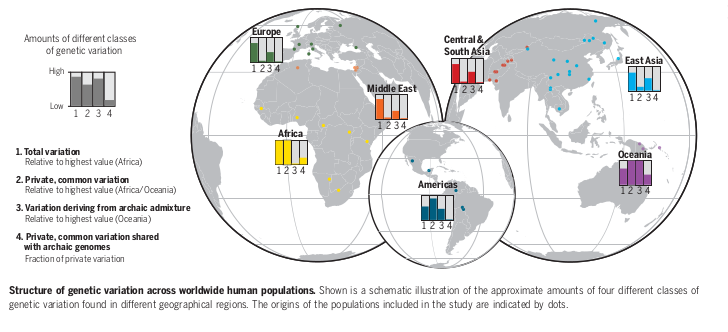
\includegraphics[width=1\textwidth]{Fig/HGDP.png}
\decoRule
\caption{}
\label{fig:HGDP}
\end{figure}

\section{Mitochondrial Genomes}
\subsection{Structure and function of mitochodria}
Mitochondria are a membrane-bound organelle present in the cytoplasm of all eukaryotic cells. They are responsible for producing Adenosine triphosphate (ATP), the main energy currency of the cell.
Mitochondria are typically round to oval in shape and range in size from 0.5 to 10 $\mu$m. In addition to producing energy, mitochondria store calcium for cell signaling activities, generate heat, and mediate cell growth and death.
Mitochondria are unlike other cellular organelles in that they have two distinct membranes and a unique genome and reproduce by binary fission. 
The outer mitochondrial membrane is freely permeable to small molecules and contains special channels capable of transporting large molecules. 
In contrast, the inner membrane is far less permeable, allowing only very small molecules to cross into the gel-like matrix that makes up the organelle’s central mass. 
The matrix contains the DNA of the mitochondrial genome (mtDNA) and the enzymes of the tricarboxylic acid (TCA) cycle (also known as the Krebs cycle), which metabolizes nutrients into by-products the mitochondrion can use for energy production. (Figure \ref{fig:Mitochondrial Function}) (\cite{friedman2014mitochondrial})

\subsection{Mitochondrial genome}
Mitochondrial DNA (mtDNA) is a double-stranded molecule of 16.6 kb. The two strands of mtDNA differ in their base composition, with one being rich in guanines, making it possible to separate a heavy (H) and a light (L) strand. The mtDNA contains one longer noncoding region (NCR) also referred to as the control region. DNA polymerase γ (POLγ) is the replicative polymerase in mitochondria. 
The circular genome contains 13 protein‐encoding sequences corresponding to subunits ND1‐6, including ND4 and ND4L, of respiratory complex I, catalytic subunits cytochrome c oxidase subunit I-III (CO1-3) of respiratory complex IV, subunits adenosine triphos-phate 6 (ATP6) and ATP8 of F1F0 ATPase, and cytochrome B of respiratory complex III. 
The remaining genes encode 22 tRNAs and 12, and 16S rRNAs. (Figure \ref{fig:Mitochondrial Genome}, \cite{stefano2016mitochondrial, garone2018mitochondrial})\\

Each human cell contains thousands of copies of mtDNA, At birth these are usually all identical (homoplasmy).
Individuals with mitochondrial disorders resulting from mutation of mtDNA may harbor a mixture of mutated and wild type mtDNA within each cell this phenomenon is called heteroplasmy. 
In many organisms, the mitochondrial genome is inherited maternally. This is because the mother’s egg cell donates the majority of cytoplasm to the embryo, and mitochondria inherited from the father’s sperm are usually destroyed but paternal mitochondrial DNA (mtDNA) transmission may coexist with maternal transmission of mtDNA. In a study on a family with mitochondrial disorders it was found that there was a high level of heteroplasmy due to paternally transmission.
  (\cite{luo2018biparental})

\begin{figure}[H]
\centering
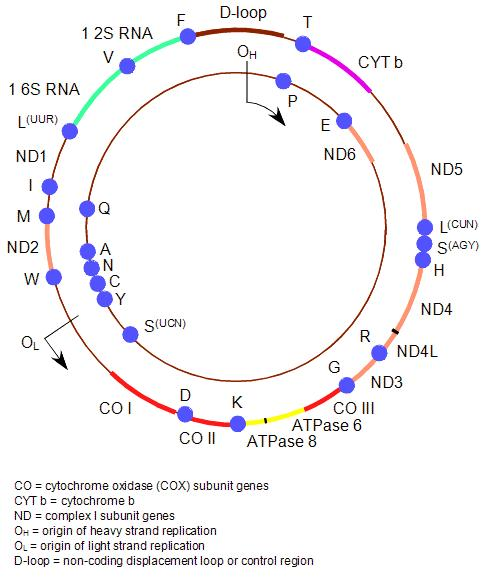
\includegraphics[width=0.7\textwidth]{Fig/mitogenome.jpg}
\decoRule
\caption{\textbf{Mitochondrial Genome}}
\label{fig:Mitochondrial Genome}
\end{figure}

\begin{figure}[H]
\centering
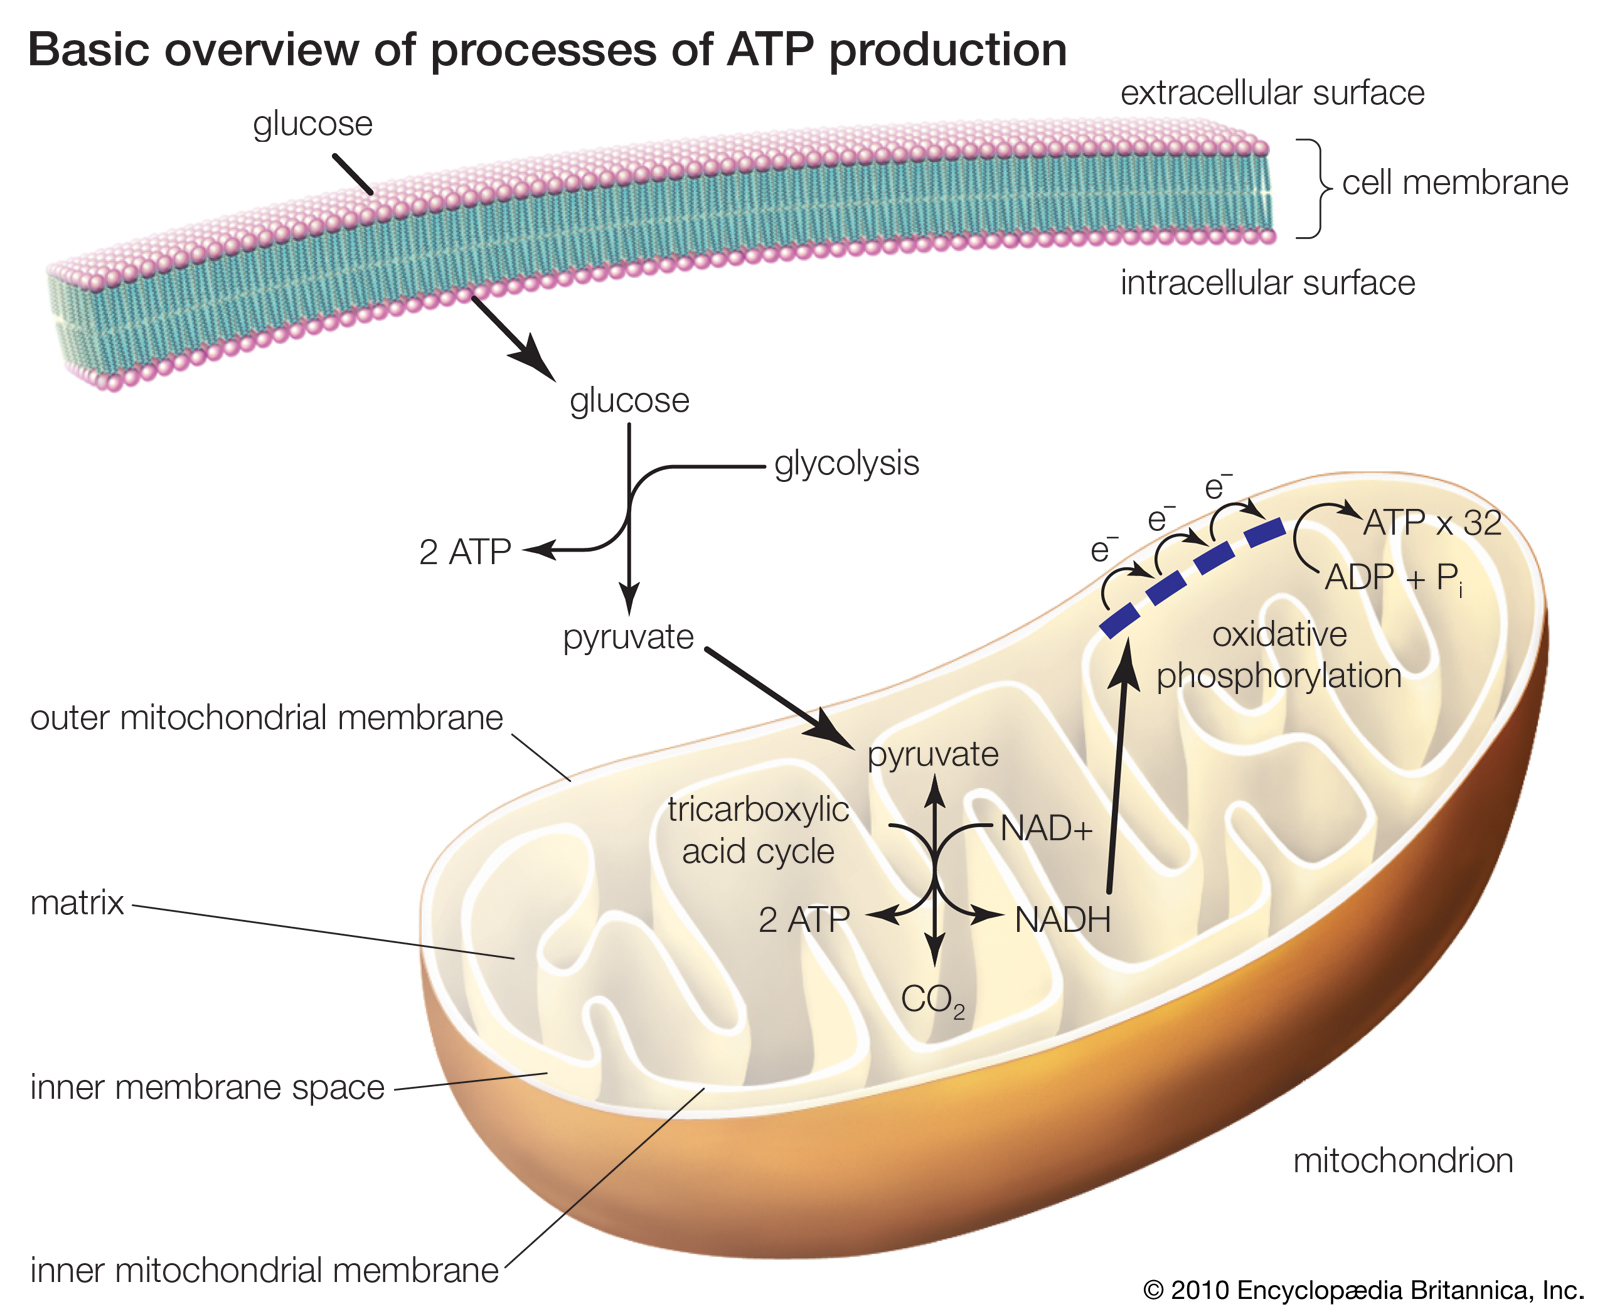
\includegraphics[width=0.7\textwidth]{Fig/processes-production-ATP-glycolysis-tricarboxylic-acid-cycle.jpg}
\decoRule
\caption{\textbf{Mitochondrial Function}}
\label{fig:Mitochondrial Function}
\end{figure}


\newline

\section{Mitochondrial mechanism encoded by nuclear genes}
Important mitochondrial mechanisms controlled by nuclear genes include
Disorders of mtDNA maintenance (mtDNA depletion or secondary pathogenic mtDNA variants), more than 1000 nuclear genes encoding mitochondrial proteins. Nuclear genes involved in mitochondrial functions are genes encoding enzymes for lipid or cofactor biosynthesis, like \textit{TAZ} (or G4.5) that encodes an acyl–coenzyme A synthetase/transacylase (tafazzin).
Most genes encoding factors involved in the assembly of the complexes of respiratory chain, like \textit{COX} genes, involved in stability and assembly of respiratory complex.
Or genes encoding factors for mitochondrial protein synthesis like the mitoribosomes encoded by \textit{MRPS22}.

(\cite{caggese1999identification} \cite{chinnery2014mitochondrial}


\section{Mitochondrial Diseases}
Mitochondrial diseases are a clinically heterogeneous group of disorders that arise as a result of dysfunction of
the mitochondrial respiratory chain.
Single-cell studies and cybrid-cell studies have shown that the proportion of mutated mtDNA must exceed a critical threshold level before a cell expresses a biochemical abnormality of the mitochondrial respiratory chain (the threshold effect). The percentage level of mutated mtDNA may vary among individuals within the same family, and also among organs and tissues within the same individual.
(\cite{chinnery2014mitochondrial} \cite{thorburn2017mitochondrial})
While some mitochondrial disorders only affect a single organ (for example the eye in Leber hereditary optic neuropathy LHON), many involve multiple organ systems and often present with prominent neurologic and myopathic features , like Leigh syndrome.
Leigh syndrome (also called Leigh disease or subacute necrotizing
encephalomyelopathy) is a rare inherited neurometabolic disorder
and affects the central nervous system. 
Genetically, alterations or mutations of the mitochondrial respiratory enzyme complex or pyruvate dehydrogenase complex are believed to be responsible for the development of Leigh syndrome.
Brainstem dysfunction manifests as respiratory symptoms and abnormalities in swallowing, ophthalmology, and thermoregulation. 
The neurologic manifestations may begin in infancy or early
childhood, progressively worsen, and eventually lead to death in
early childhood ; Leigh syndrome can also occur at any age, including adolescence or adulthood.
(\cite{chang2020meta})


%\section{Hypothesis testing}
%Mannwithney 
%F-test 
\section{project GREP}
The work I have done during my thesis is part of the project \textit{Genomics of REcurrent Pregnancy loss (GREP)} lead by the Institute of Genetics and Biophysics of the National Research Council in collaboration with the University of Napoli Federico II, and several other partners in Italy, United Kingdom, Malaysia, Pakistan, and Australia.  

GREP aims to identify genetic variants likely to cause PL not seen by current diagnostic tools (mainly comparative genomic hybridization), either because of the size or because they are located in non-coding regions not considered in medical diagnostics. The main objective of GREP is to build a predictive model that integrates genomic variation and functional annotations, based on the analysis of whole-genome sequences of miscarried embryos.\\

\chapter{Aim of the project }
The aim of this study is to identify genomic variants likely to cause idiopathic pregnancy losses that are not seen by current diagnostic tools either because of their very small size or because they lie in non-coding regulatory regions of the genome that are not routinely sequenced.

The expectation is to identify highly deleterious dominant \textit{de novo} mutations in sporadic cases and rare moderately deleterious recessive mutations in homozygosis or compound heterozygosity in recurrent pregnancy losses 

objectives 
- study embryonic mitochondrial sequences from recurrent miscarriages in humans.
- identify variants potentially detrimental 
- identify genes potentially involved
